% vim: textwidth=99 spell spelllang=en_gb:
\graphicspath{{graphics/}} % set of paths to search for images
\DeclareGraphicsExtensions{.pdf,.png}

\appendix
\setboolean{@mainmatter}{true}

\chapter{Interfaces and Enums}%
\label{cha:interfaces_and_enums}

\begin{verbatim}
enum ETincture {
  /** For specifying Quarters */
  Quarterly = "quarterly",
  /** Gold/yellow */
  Or = "or",
  /** White */
  Argent = "argent",
  /** Blue */
  Azure = "azure",
  /** Red */
  Gules = "gules",
  /** Purple */
  Purpure = "purpure",
  /** Black */
  Sable = "sable",
  /** Green */
  Vert = "vert",
}

enum ECharge {
  Bend = "bend",
  Cross = "cross",
  Chief = "chief",
  Saltire = "saltire",
}

enum EQuarter {
  TL = "quarterly_tl",
  TR = "quarterly_tr",
  BL = "quarterly_bl",
  BR = "quarterly_br",
}

interface ICharge {
  charge: ECharge;
  sinister?: boolean;
  tincture?: ETincture;
}

interface IBlazon {
  field: ETincture;
  charges: ICharge[];
}
\end{verbatim}

\chapter{UML Diagrams}%
\label{cha:uml_diagrams}

In these UML diagrams, \texttt{d3.Selection} is a data type defined by D3.js~\autocite{d3js}. It
contains a reference to an HTML element for use in \dom{} manipulation.

\section{Second Design Iteration Diagrams}%
\label{sec:second_design_iteration_diagrams}

\begin{figure*}[h]
  %\centering
  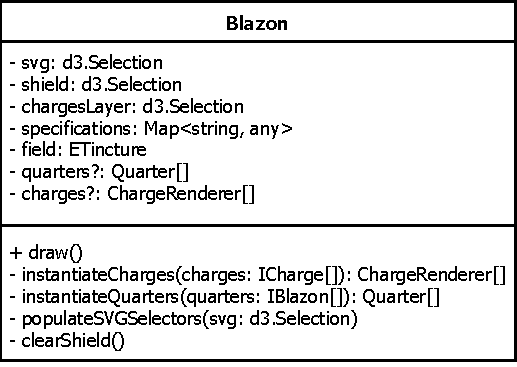
\includegraphics[width=0.5\linewidth]{BlazonUML}
  \caption{\texttt{Blazon} UML.}%
  \label{fig:BlazonUML}
\end{figure*}

\begin{figure*}[h]
  %\centering
  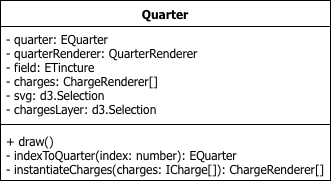
\includegraphics[width=0.5\linewidth]{QuarterUML}
  \caption{\texttt{Quarter} UML.}%
  \label{fig:QuarterUML}
\end{figure*}

\begin{figure*}[h]
  %\centering
  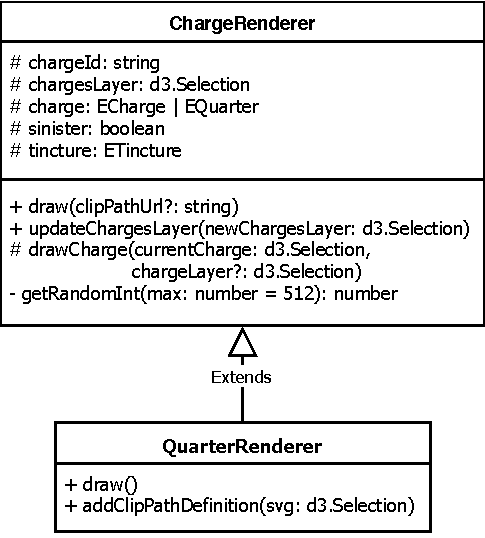
\includegraphics[width=0.5\linewidth]{ChargeRendererUML}%
  \caption{\texttt{ChargeRenderer} hierarchy and methods.}%
  \label{fig:charge_renderer_heirarchy}
\end{figure*}

\pagebreak%

\section{Third Design Iteration Diagrams}%
\label{sec:third_design_iteration_diagrams}

\begin{figure*}[h]
  %\centering
  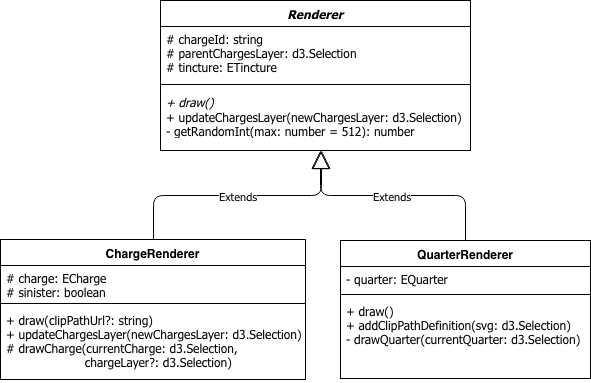
\includegraphics[width=0.8\linewidth]{RendererUML}
  \caption{\texttt{Renderer} hierarchy and methods.}%
  \label{fig:RendererUML}
\end{figure*}

\begin{figure*}[h]
  %\centering
  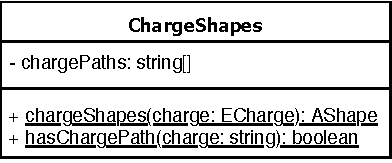
\includegraphics[width=0.5\linewidth]{ChargeShapesUML}
  \caption{\texttt{ChargeShapes} UML.}%
  \label{fig:ChargeShapesUML}
\end{figure*}

\begin{figure*}[h]
  %\centering
  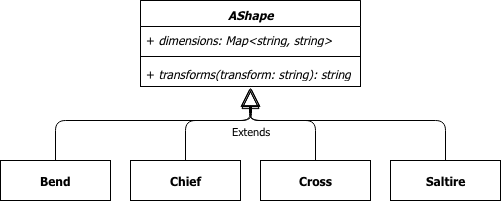
\includegraphics[width=0.8\linewidth]{AShapeUML}
  \caption{\texttt{AShape} hierarchy and methods.}%
  \label{fig:AShapeUML}
\end{figure*}

\setboolean{@mainmatter}{false}
